\documentclass[conference]{IEEEtran}

% ============================================================
% IEEE-style paper skeleton
% Project: Rice leaf disease classification with lightweight CNN,
% segmentation, and explicit texture features
% ============================================================

% --- Encoding and language ---
\usepackage[utf8]{inputenc}
\usepackage[T1]{fontenc}
\usepackage[english]{babel}

% --- Mathematics ---
\usepackage{amsmath, amssymb, amsfonts}

% --- Figures and tables ---
\usepackage{graphicx}
\usepackage{booktabs}
\usepackage{multirow}
\usepackage{array}
\usepackage{tabularx}
\usepackage{makecell}
\usepackage{siunitx}
\usepackage{adjustbox}

% --- Algorithms / pseudo-code if needed later ---
\usepackage{algorithm}
\usepackage{algorithmic}

% --- References and hyperlinks ---
\usepackage{cite}
\usepackage[hidelinks]{hyperref}
\usepackage{xurl}

% --- Utility ---
\usepackage{xcolor}
\usepackage{balance}

% --- IEEE configuration ---
\IEEEoverridecommandlockouts
\sisetup{detect-weight=true, detect-family=true}

% --- Custom commands ---
\newcommand{\modelbase}{E0}
\newcommand{\modelseg}{E1}
\newcommand{\modeltex}{E2}
\newcommand{\modelprop}{E3}
\newcommand{\macroF}{Macro-F1}
\newcommand{\todo}[1]{\textcolor{red}{[TODO: #1]}}

\begin{document}

\title{Controlled Ablation Evaluation of Segmentation and Explicit Texture Features in Lightweight CNNs for Rice Leaf Disease Classification}

\author{%
\IEEEauthorblockN{D'Alessandro del Piero Sarmiento Ayala}
\IEEEauthorblockA{Universidad San Ignacio de Loyola\\
Course: Mathematics Applied to Computing\\
Instructor: Dr. Manuel Augusto Yarleque Medina\\
Email: \href{mailto:d.sarmiento@usil.pe}{d.sarmiento@usil.pe}\\
ORCID: \href{https://orcid.org/0009-0005-1480-1671}{0009-0005-1480-1671}}
}

\maketitle

\begin{abstract}
Rice leaf diseases require timely visual diagnosis because they can affect crop productivity and disease management decisions. Recent convolutional neural networks (CNNs) and transfer learning models have achieved strong performance in plant disease recognition; however, RGB-based classification may still be influenced by background conditions, illumination variability, or dataset-specific visual patterns. This paper presents an applied, quantitative, experimental, and descriptive-comparative study that evaluates the contribution of classical segmentation and explicit texture descriptors in lightweight CNN-based rice leaf disease classification. Four configurations were compared: a MobileNetV2 baseline trained on original RGB images, a CNN trained on segmented images, a CNN fused with explicit texture features, and a hybrid configuration combining segmentation and texture features. The dataset split was controlled using perceptual-hash grouping to avoid visually equivalent samples across training, validation, and test sets. Experiments were repeated across five random seeds and evaluated using accuracy, macro-precision, macro-recall, macro-F1, inference time, model size, and parameter count. The texture-fusion configuration obtained the highest mean macro-F1 score of 0.9993, followed by the segmentation-only model with 0.9976, the proposed hybrid model with 0.9976, and the baseline with 0.9969. Although the enhanced configurations achieved higher average scores than the baseline, the differences were not statistically significant across five seeds. These results suggest that texture and segmentation are useful components for controlled ablation, but the dataset presents a performance saturation scenario in which several lightweight configurations already achieve very high classification performance.
\end{abstract}

\begin{IEEEkeywords} Rice leaf disease classification, lightweight CNN, MobileNetV2, image segmentation, GLCM, DWT, texture features, ablation study, perceptual hash. \end{IEEEkeywords}

\section{Introduction}

Rice is one of the most important staple crops worldwide and plays a central role in food security, particularly in regions where it represents a major source of daily caloric intake. The Food and Agriculture Organization reports that rice is the staple food for more than half of the world's population, and that in Asia more than two billion people obtain a large share of their caloric intake from rice and rice-derived products \cite{fao_rice_conference}. Therefore, the early identification of rice diseases is relevant not only for agronomic management but also for protecting crop productivity in rice-dependent regions.

Rice production is affected by several foliar diseases, including blast, bacterial blight, brown spot, and tungro. The International Rice Research Institute identifies disease damage as a factor that can greatly reduce rice yield and describes tungro as one of the most destructive diseases of rice in South and Southeast Asia \cite{irri_rice_diseases,irri_rice_disease_damage}. These diseases manifest through visual symptoms such as spots, lesions, discoloration, necrosis, or leaf deformation, making image-based diagnosis a feasible computer vision task. However, visual symptoms may also vary with plant stage, lighting, image acquisition conditions, and disease severity, which can complicate automatic classification.

Traditional plant disease diagnosis commonly depends on manual inspection, field observation, or expert assessment. Although this process is useful in practice, it can be time-consuming, labor-intensive, subjective, and difficult to scale for large agricultural areas. As a result, computer vision and machine learning methods have become increasingly relevant for supporting automatic crop disease recognition. Public image datasets, such as the Rice Leaf Disease Images dataset used in this study, provide labeled samples for bacterial blight, blast, brown spot, and tungro, enabling supervised experimentation with deep learning models \cite{kaggle_rice_leaf_disease}.

Convolutional neural networks and transfer learning have shown strong performance in plant disease recognition. In rice disease classification, architectures based on DenseNet121 and other deep models have reported high predictive performance \cite{ismail2026densenet}. Lightweight detection models have also been proposed to balance performance and computational cost, as in RiceDetect-Net, which focuses on real-time rice disease detection \cite{yuan2026ricedetectnet}. These studies demonstrate that deep visual representations can capture discriminative patterns from diseased leaves. Nevertheless, high in-distribution accuracy does not always imply that a model is using only disease-related visual cues. Deep neural networks may exploit shortcut features or spurious correlations that perform well on a benchmark but generalize poorly under more challenging conditions \cite{geirhos2020shortcut}. In plant disease datasets, this concern is especially relevant because background, acquisition conditions, and dataset-specific artifacts may correlate with class labels \cite{noyan2022plantvillage_bias}.

Several research lines attempt to reduce these limitations by incorporating segmentation or explicit handcrafted descriptors. Segmentation-based approaches aim to isolate the leaf or lesion region so that the classifier focuses on more relevant visual information. For example, contour-driven segmentation has been used to improve rice leaf disease classification with transfer learning architectures \cite{shakeel2026contour}, while automatic segmentation and multi-scale feature fusion have been explored for plant disease detection in complex backgrounds \cite{arora2025complex}. In a different but complementary direction, explicit texture descriptors such as gray-level co-occurrence matrix (GLCM), local binary patterns (LBP), color histograms, and frequency-domain descriptors have been used to represent local texture, spatial intensity relationships, and color distributions. Feature fusion using GLCM, LBP, and color histograms has been proposed for rice leaf disease classification \cite{sutikno2026glcm_lbp_color}, supporting the idea that handcrafted descriptors can still provide useful information for disease recognition.

However, the reviewed literature suggests that these components are often studied separately, embedded in complex architectures, or evaluated without isolating their individual and combined contributions under the same lightweight CNN protocol. CNN-based works tend to prioritize final predictive accuracy, segmentation-based works often focus on region extraction or complex pipelines, and texture-based works frequently rely on handcrafted feature fusion or traditional classifiers. Consequently, there remains a practical methodological gap: it is not sufficiently clear whether classical segmentation, explicit texture descriptors, or their combination with CNN embeddings provide measurable benefits over a lightweight CNN baseline when evaluated under a controlled ablation study for rice leaf disease classification.

To address this gap, this paper evaluates four configurations using a common dataset, split strategy, training setup, and evaluation protocol: (i) a MobileNetV2 baseline trained on original RGB images, (ii) a CNN trained on segmented images, (iii) a CNN fused with explicit texture features, and (iv) a hybrid configuration combining segmentation and texture features.

The main contributions of this work are summarized as follows:
\begin{itemize}
    \item A controlled ablation study comparing RGB input, segmentation, explicit texture features, and segmentation-texture fusion in lightweight CNN-based rice leaf disease classification.
    \item A leakage-aware dataset partitioning procedure based on perceptual-hash grouping to avoid visually equivalent samples across training, validation, and test sets.
    \item A multi-seed evaluation protocol reporting mean and standard deviation for macro-F1, accuracy, precision, recall, inference time, parameter count, and model size.
    \item A critical interpretation of whether segmentation and texture features improve predictive performance or mainly add complexity under a high-performing lightweight CNN baseline.
\end{itemize}

The remainder of this paper is organized as follows. Section II reviews related work on rice leaf disease classification, segmentation-based recognition, and explicit texture descriptors. Section III describes the research design, dataset, leakage control, experimental scenarios, and evaluation protocol. Section IV presents the preprocessing, segmentation, feature extraction, model architecture, and implementation details. Section V reports the experimental results. Section VI discusses the findings, limitations, and methodological implications. Finally, Section VII presents the conclusions and future work.


\section{Related Work}

\subsection{Deep Learning for Rice Disease Classification}

Deep learning and transfer learning have become common approaches for rice disease classification because they can learn discriminative visual patterns directly from leaf images. A DenseNet121-based model for rice plant disease classification reported an average testing accuracy of 97.9\%, showing that pre-trained CNN backbones can provide strong performance in this domain \cite{ismail2026densenet}. This result is relevant to the present study because it confirms that CNN-based models are already strong baselines for rice disease recognition. However, such works mainly evaluate the final predictive capacity of a deep architecture, rather than isolating the contribution of classical preprocessing or handcrafted descriptors under the same experimental protocol.

\subsection{Segmentation-Aware Plant Disease Recognition}

Segmentation-aware approaches attempt to reduce the influence of background and irrelevant visual regions by focusing the classifier on the leaf or lesion area. A contour-driven segmentation approach combined with optimized transfer learning architectures achieved 98.43\% test accuracy and 98.70\% F1-score for rice leaf disease classification \cite{shakeel2026contour}. This antecedent is directly related to the segmentation component of the present work, since both approaches use region-focused processing before classification. Nevertheless, the cited study evaluates segmentation as part of a larger optimized transfer learning pipeline, while this paper evaluates segmentation as an isolated ablation factor against an RGB baseline and texture-based variants.

\subsection{Explicit Texture and Hybrid Feature Descriptors}

Texture-based descriptors remain relevant in rice disease classification because symptoms such as spots, lesions, necrotic regions, and discoloration can be represented through spatial intensity relationships and local texture patterns. A feature-fusion method combining GLCM, LBP, and color histograms achieved 97.22\% accuracy on RLD1 and 99.41\% on RLD2, outperforming several individual descriptor combinations \cite{sutikno2026glcm_lbp_color}. Similarly, a hybrid feature extraction approach based on GLCM, GLDM, texture, FFT, and DWT features with a feed-forward neural network achieved an average accuracy of 94.84 $\pm$ 0.04\%, with the authors also reporting statistical validation through a paired test \cite{prity2026ffnn}. These studies support the use of explicit handcrafted descriptors for capturing complementary information, especially texture and frequency patterns that may not be explicitly controlled in standard CNN pipelines.

Overall, previous studies show that CNN backbones, segmentation-aware processing, and handcrafted texture or frequency descriptors can each improve plant or rice disease recognition. However, they are usually evaluated as independent solutions or as part of broader optimized architectures. This makes it difficult to determine the individual and combined contribution of segmentation and explicit texture features when integrated with a lightweight CNN. Therefore, this paper focuses on a controlled ablation study that compares four configurations under the same dataset split, training setup, metrics, and multi-seed evaluation protocol: RGB baseline, segmented-input CNN, CNN with texture fusion, and a segmentation-texture hybrid model.

\section{Methodology}

\subsection{Research Design and Methodological Framework}

This study was designed as a controlled ablation study for supervised rice leaf disease classification. The methodological framework follows an applied quantitative experimental approach: a computational pipeline was implemented, the input-processing configuration was deliberately modified across experimental scenarios, and the resulting models were compared using numerical performance and efficiency metrics.

The ablation design was selected to isolate the contribution of each component under comparable conditions. Instead of evaluating only a final proposed architecture, the study compared a baseline CNN, a segmentation-based variant, a texture-fusion variant, and a segmentation-texture hybrid variant. To ensure a fair comparison, all scenarios used the same dataset split, image size, training configuration, evaluation metrics, and random seeds. Therefore, the intended experimental factor was the presence or absence of segmentation and explicit texture descriptors.

\subsection{Dataset and Split Distribution}

The experiments used the Rice Leaf Disease Images dataset, organized into four disease classes: Bacterial Blight, Blast, Brown Spot, and Tungro. The final dataset contained 5,932 images. The dataset was divided into training, validation, and test sets following an approximate 70\%--15\%--15\% distribution. The training set contained 4,150 images, representing 69.96\% of the dataset; the validation set contained 891 images, representing 15.02\%; and the test set contained 891 images, also representing 15.02\%. Table~\ref{tab:split_distribution} shows the final class distribution.

\begin{table}[t]
\caption{Dataset split distribution by class.}
\label{tab:split_distribution}
\centering
\footnotesize
\setlength{\tabcolsep}{4pt}
\begin{tabular}{lccc}
\toprule
Class & Train & Val. & Test \\
\midrule
Bacterial Blight & 1108 & 238 & 238 \\
Blast            & 1007 & 216 & 217 \\
Brown Spot       & 1120 & 241 & 239 \\
Tungro           & 915  & 196 & 197 \\
\midrule
Total            & 4150 & 891 & 891 \\
Percentage       & 69.96\% & 15.02\% & 15.02\% \\
\bottomrule
\end{tabular}
\end{table}

\subsection{Data Leakage Control Using Perceptual Hashing}

A preliminary inspection showed that the dataset contained visually repeated or highly similar samples. To reduce the risk of data leakage, the final partition was generated using perceptual hash grouping. Each image was assigned a perceptual hash, and images sharing the same hash were kept within the same split.

After this correction, the dataset contained 2,927 unique perceptual hashes across 5,932 images. The number of perceptual hashes appearing in more than one split was zero. This procedure was applied before training to avoid inflated validation or test performance caused by visually equivalent samples shared across training, validation, and test subsets.

\subsection{Experimental Scenarios}

Four scenarios were evaluated. E0 was the baseline model trained with original RGB images. E1 evaluated the effect of replacing the original RGB image with its segmented version. E2 evaluated the effect of fusing MobileNetV2 image embeddings with explicit GLCM+DWT features extracted from original images. E3 was the proposed hybrid variant, combining segmented images with GLCM+DWT features extracted from the segmented image source. Table~\ref{tab:scenarios} summarizes the four ablation scenarios evaluated in the study.

\begin{table}[t]
\caption{Ablation scenarios evaluated in the study.}
\label{tab:scenarios}
\centering
\footnotesize
\setlength{\tabcolsep}{3pt}
\begin{tabularx}{\columnwidth}{c X X}
\toprule
ID & Configuration & Purpose \\
\midrule
E0 & MobileNetV2 + original RGB image & Baseline \\
E1 & MobileNetV2 + segmented image & Segmentation effect \\
E2 & MobileNetV2 + original image + GLCM+DWT & Texture fusion effect \\
E3 & MobileNetV2 + segmented image + GLCM+DWT & Proposed hybrid variant \\
\bottomrule
\end{tabularx}
\end{table}

\subsection{Evaluation Protocol}

The primary evaluation metric was macro-F1, selected because it gives equal importance to all classes. Additional metrics included accuracy, macro-precision, macro-recall, confusion matrix, inference time per image, number of parameters, and model size.

To evaluate stability, the complete training process was repeated using five random seeds: 42, 123, 2026, 7, and 99. This produced 20 total runs, corresponding to four experimental scenarios evaluated across five seeds. Final performance was summarized using the mean and standard deviation across seeds.

Since the same seeds were used for all scenarios, pairwise differences against the baseline were computed by seed. The Wilcoxon signed-rank test was used to assess whether the macro-F1 differences between each enhanced scenario and the baseline were statistically significant without assuming normality of the paired differences.

Figure~\ref{fig:experimental_framework} summarizes the complete experimental workflow, including dataset preparation, leakage control, ablation scenarios, model training, evaluation metrics, and comparative analysis.

\begin{figure*}[!t]
\centering
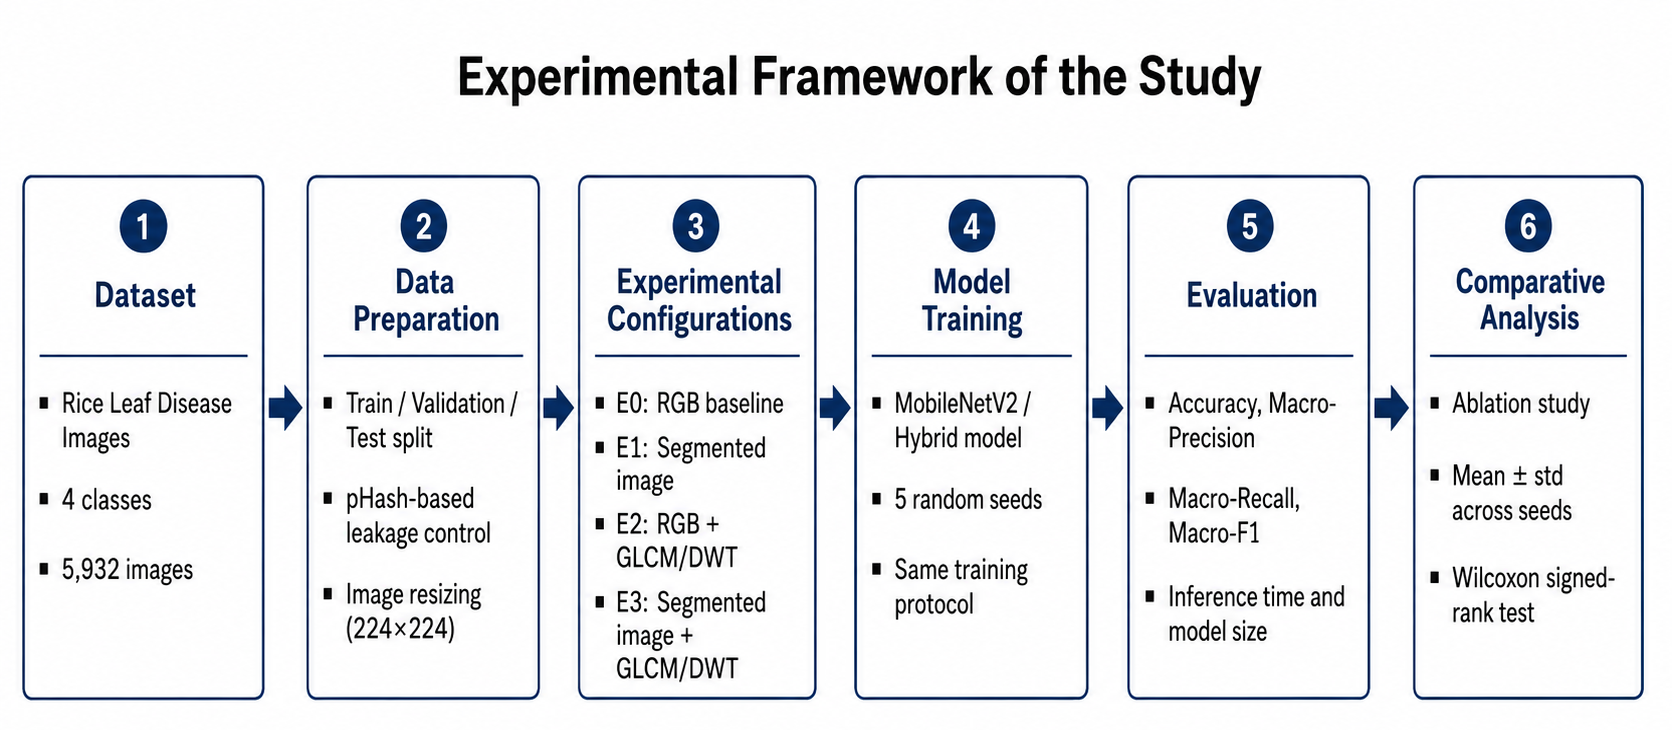
\includegraphics[width=0.88\textwidth]{figures/fig01_experimental_framework.png}
\caption{Experimental framework and ablation scenarios evaluated in this study.}
\label{fig:experimental_framework}
\end{figure*}

\section{Experimental Development}

\subsection{Preprocessing and Segmentation}

All images were resized to $224 \times 224$ pixels before being used by the CNN, segmentation module, or handcrafted feature extractor. For the segmentation-based scenarios, each RGB image was converted to the L*a*b* color space. The binary region-of-interest mask was generated from the $a$ channel using Otsu thresholding \cite{otsu1979threshold}. This channel was selected because it captures the green-red chromatic component, which is useful for separating leaf and lesion regions from parts of the background.

The resulting binary mask was refined using morphological opening and closing with a kernel size of 5. Pixels outside the mask were replaced by zero, producing a segmented image. Given an input image $I$ and a binary mask $M$, the segmented image $I_s$ was computed as:

\begin{equation}
I_s(x,y) =
\begin{cases}
I(x,y), & \text{if } M(x,y)=1,\\
0, & \text{otherwise.}
\end{cases}
\end{equation}

This segmentation strategy was used for E1 and E3. In E1, the segmented image was passed directly to MobileNetV2. In E3, the segmented image was used both as CNN input and as the source for extracting handcrafted texture and frequency features.

\subsection{Texture Feature Extraction}

Explicit handcrafted descriptors were extracted from original images for E2 and from segmented images for E3. The feature extractor combined gray-level co-occurrence matrix (GLCM) descriptors and discrete wavelet transform (DWT) descriptors.

The GLCM descriptors represented spatial gray-level relationships using contrast, dissimilarity, homogeneity, energy, correlation, and angular second moment (ASM) \cite{haralick1973glcm}. For each descriptor, the mean and standard deviation were computed, producing 12 texture features.

The DWT descriptors represented multiresolution frequency information \cite{mallat1989wavelet}. Mean, standard deviation, energy, and entropy were extracted from the approximation coefficients and from horizontal, vertical, and diagonal detail coefficients at two decomposition levels. This produced 28 frequency-domain features. Therefore, each image used in the texture-based scenarios was represented by 40 numerical handcrafted descriptors: 12 GLCM-based features and 28 DWT-based features.

Before training the hybrid models, the handcrafted feature vectors were standardized using a \texttt{StandardScaler}. The scaler was fitted only on the training split and then applied to the validation and test splits, preventing information leakage during normalization.

\subsection{Model Architecture}

The image backbone was MobileNetV2 with ImageNet pre-trained weights \cite{sandler2018mobilenetv2}. For E0 and E1, the original classifier head was replaced by a dropout layer followed by a fully connected layer with four output units, corresponding to the four disease classes. The backbone was fine-tuned during training.

For E2 and E3, a two-branch hybrid architecture was implemented. The first branch extracted an image embedding using MobileNetV2 followed by adaptive average pooling. The second branch processed the standardized 40-dimensional handcrafted feature vector through a fully connected layer with 128 hidden units, ReLU activation, and dropout. The image embedding and texture representation were concatenated and passed to a fusion classifier with 256 hidden units, ReLU activation, dropout, and a final four-class output layer.

Figure~\ref{fig:proposed_hybrid_architecture} illustrates the proposed E3 architecture. In this configuration, the segmented image is used both as the CNN input and as the source for explicit GLCM+DWT feature extraction, making the fusion between segmentation and handcrafted descriptors explicit.

\begin{figure}[!t]
\centering
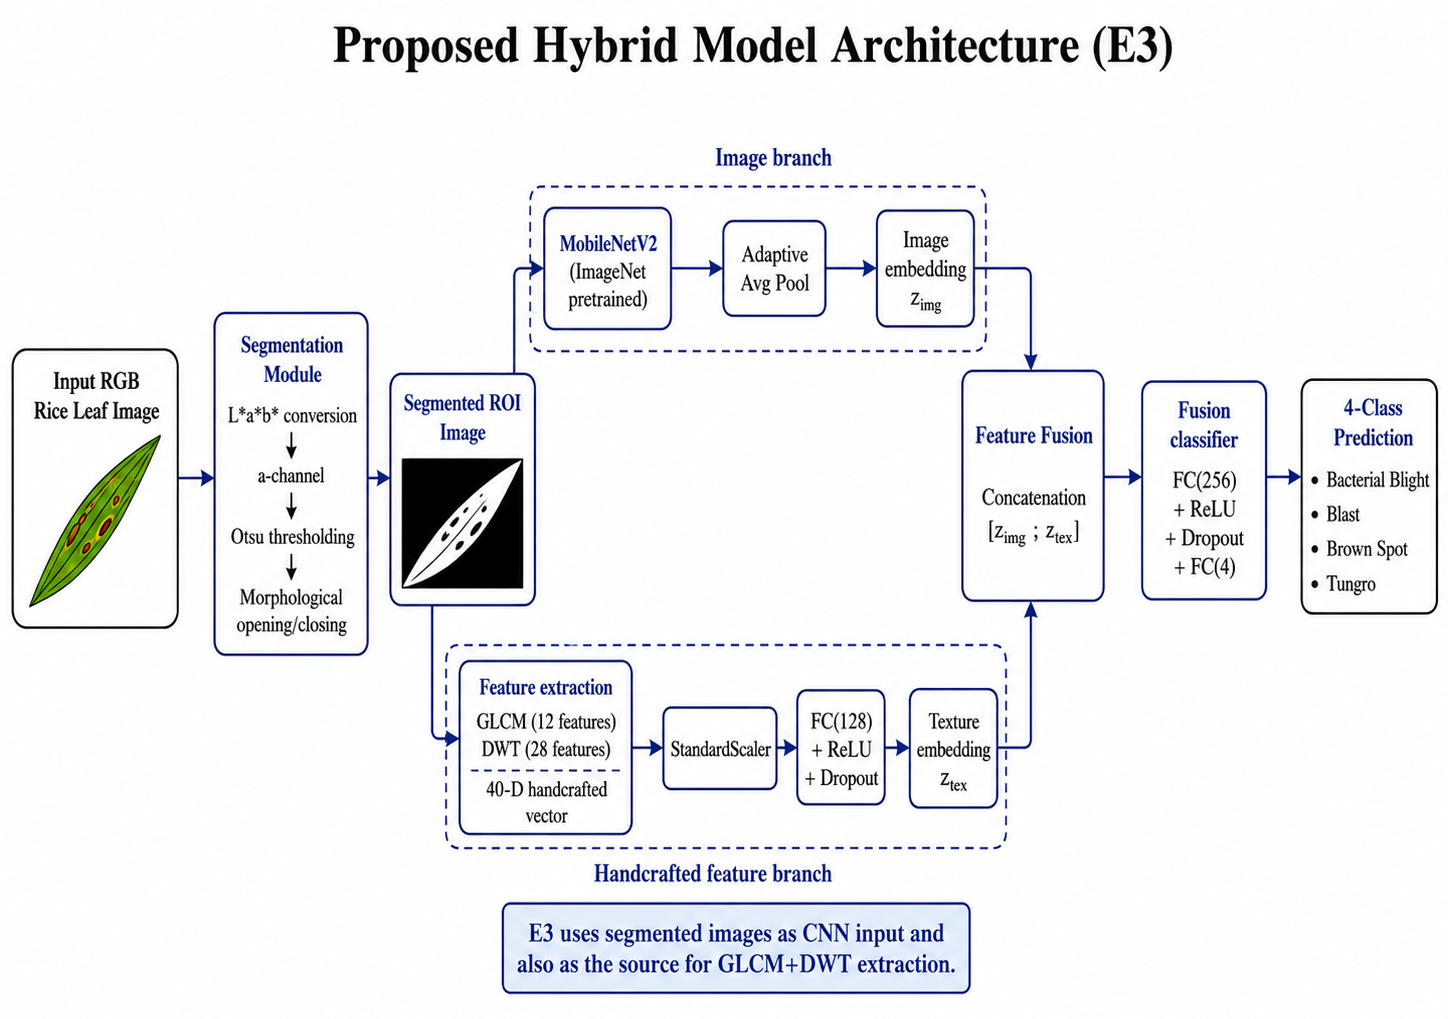
\includegraphics[width=\columnwidth]{figures/fig02_proposed_hybrid_architecture_e3.png}
\caption{Proposed hybrid model architecture for E3.}
\label{fig:proposed_hybrid_architecture}
\end{figure}

Let $\mathbf{z}_{img}$ denote the MobileNetV2 image embedding and $\mathbf{z}_{tex}$ denote the learned representation of the handcrafted feature vector. The fused representation is defined as:

\begin{equation}
\mathbf{z}_{fused} = [\mathbf{z}_{img}; \mathbf{z}_{tex}],
\end{equation}

where $[\,;\,]$ denotes vector concatenation. The final class prediction is obtained by applying the fusion classifier to $\mathbf{z}_{fused}$.


\subsection{Training Configuration and Implementation Details}

All models were trained with the same configuration: 30 maximum epochs, batch size of 8, AdamW optimizer, learning rate of $1 \times 10^{-4}$, weight decay of $1 \times 10^{-4}$, cosine learning-rate scheduler, and early stopping with patience of 7 based on validation macro-F1.

The implementation was developed in Python using PyTorch for model training, OpenCV for image processing and segmentation, scikit-image and PyWavelets for feature extraction, and scikit-learn for feature standardization and evaluation utilities. The experiments were executed on an NVIDIA GeForce RTX 3050 Laptop GPU with CUDA support.
\section{Results}

\subsection{Multi-Seed Performance}

Table~\ref{tab:multiseed} summarizes the performance of the four experimental scenarios over five random seeds. The CNN with texture fusion (E2) obtained the highest average performance, with a macro-F1 of $0.9993 \pm 0.0015$ and an accuracy of $0.9993 \pm 0.0015$. The segmentation-only model (E1) achieved a macro-F1 of $0.9976 \pm 0.0029$, while the proposed segmentation-texture hybrid model (E3) achieved a similar macro-F1 of $0.9976 \pm 0.0035$. The baseline CNN (E0) obtained the lowest average macro-F1, with $0.9969 \pm 0.0052$.

Although all models achieved high classification performance, the results show different trade-offs. E2 obtained the best average macro-F1, but it required more parameters and a larger model size than E0 and E1. E1 achieved the lowest average inference time, with $2.7714 \pm 0.4108$ ms/image, while maintaining high predictive performance. E3 remained competitive, but it did not outperform E2 in average macro-F1 and had a larger model size than the non-texture CNN variants.

\begin{table*}[t]
\caption{Multi-seed summary over five runs. Values are reported as mean $\pm$ standard deviation.}
\label{tab:multiseed}
\centering
\footnotesize
\begin{adjustbox}{width=\textwidth}
\begin{tabular}{lccccccc}
\toprule
Model & Accuracy & Macro-Precision & Macro-Recall & Macro-F1 & Inference (ms/img) & Parameters & Size (MB) \\
\midrule
E0 Baseline CNN &
$0.9969 \pm 0.0053$ &
$0.9970 \pm 0.0052$ &
$0.9969 \pm 0.0053$ &
$0.9969 \pm 0.0052$ &
$3.9542 \pm 0.7074$ &
2.23M &
8.74 \\

E1 Segmented CNN &
$0.9975 \pm 0.0030$ &
$0.9977 \pm 0.0027$ &
$0.9975 \pm 0.0030$ &
$0.9976 \pm 0.0029$ &
$2.7714 \pm 0.4108$ &
2.23M &
8.74 \\

E2 CNN + Texture &
$\mathbf{0.9993 \pm 0.0015}$ &
$\mathbf{0.9994 \pm 0.0014}$ &
$\mathbf{0.9993 \pm 0.0015}$ &
$\mathbf{0.9993 \pm 0.0015}$ &
$4.3820 \pm 0.7072$ &
2.59M &
10.12 \\

E3 Segmented CNN + Texture &
$0.9975 \pm 0.0036$ &
$0.9977 \pm 0.0033$ &
$0.9975 \pm 0.0037$ &
$0.9976 \pm 0.0035$ &
$3.5657 \pm 0.7854$ &
2.59M &
10.12 \\
\bottomrule
\end{tabular}
\end{adjustbox}
\end{table*}

\subsection{Statistical Comparison Against the Baseline}

To evaluate whether the enhanced configurations produced consistent improvements over the baseline, paired macro-F1 differences were computed against E0 using the same five seeds. Table~\ref{tab:statistical_comparison} reports the mean macro-F1 deltas and Wilcoxon signed-rank test results.

E2 obtained the largest average improvement over E0, with a mean macro-F1 delta of $+0.0024$. E1 and E3 also showed positive average deltas, with $+0.0007$ and $+0.0007$, respectively. However, the Wilcoxon signed-rank test did not indicate statistically significant differences for any enhanced scenario. The obtained $p$-values were 1.00 for E1 versus E0, 0.75 for E2 versus E0, and 1.00 for E3 versus E0. Therefore, although the enhanced variants improved the average macro-F1, these differences were not statistically significant under the five-seed evaluation.

\begin{table}[t]
\caption{Paired macro-F1 comparison against the baseline.}
\label{tab:statistical_comparison}
\centering
\footnotesize
\setlength{\tabcolsep}{4pt}
\begin{tabular}{lccc}
\toprule
Comparison & $\Delta$ Macro-F1 & Std. & $p$-value \\
\midrule
E1 -- E0 & $+0.0007$ & 0.0069 & 1.00 \\
E2 -- E0 & $+0.0024$ & 0.0059 & 0.75 \\
E3 -- E0 & $+0.0007$ & 0.0057 & 1.00 \\
\bottomrule
\end{tabular}
\end{table}

\subsection{Aggregate Confusion Matrix Analysis}

To complement the metric-based evaluation, confusion matrices were aggregated across the five seeds for each model. Since each seed was evaluated on 891 test images, each aggregate confusion matrix summarizes 4,455 predictions per experimental scenario.

The aggregate results confirm the trend observed in Table~\ref{tab:multiseed}. The baseline model (E0) produced 4,441 correct predictions and 14 errors, corresponding to an aggregate accuracy of 0.9969. The texture-fusion model (E2) produced 4,452 correct predictions and only 3 errors, corresponding to the highest aggregate accuracy of 0.9993. The proposed hybrid model (E3) produced 4,444 correct predictions and 11 errors, corresponding to an aggregate accuracy of 0.9975. Therefore, E3 improved over the baseline in aggregate accuracy, but E2 remained the strongest configuration overall.

Figure~\ref{fig:aggregate_confusion_matrices} compares the aggregate confusion matrices for E0, E2, and E3. E0 is included as the baseline reference, E2 is included because it obtained the highest average macro-F1 and the lowest number of aggregate errors, and E3 is included because it corresponds to the proposed segmentation-texture hybrid architecture. The aggregate matrices show that most errors occurred among visually similar disease classes, while Tungro remained highly stable across the evaluated configurations.

\begin{figure*}[t]
\centering
\begin{minipage}{0.32\textwidth}
\centering
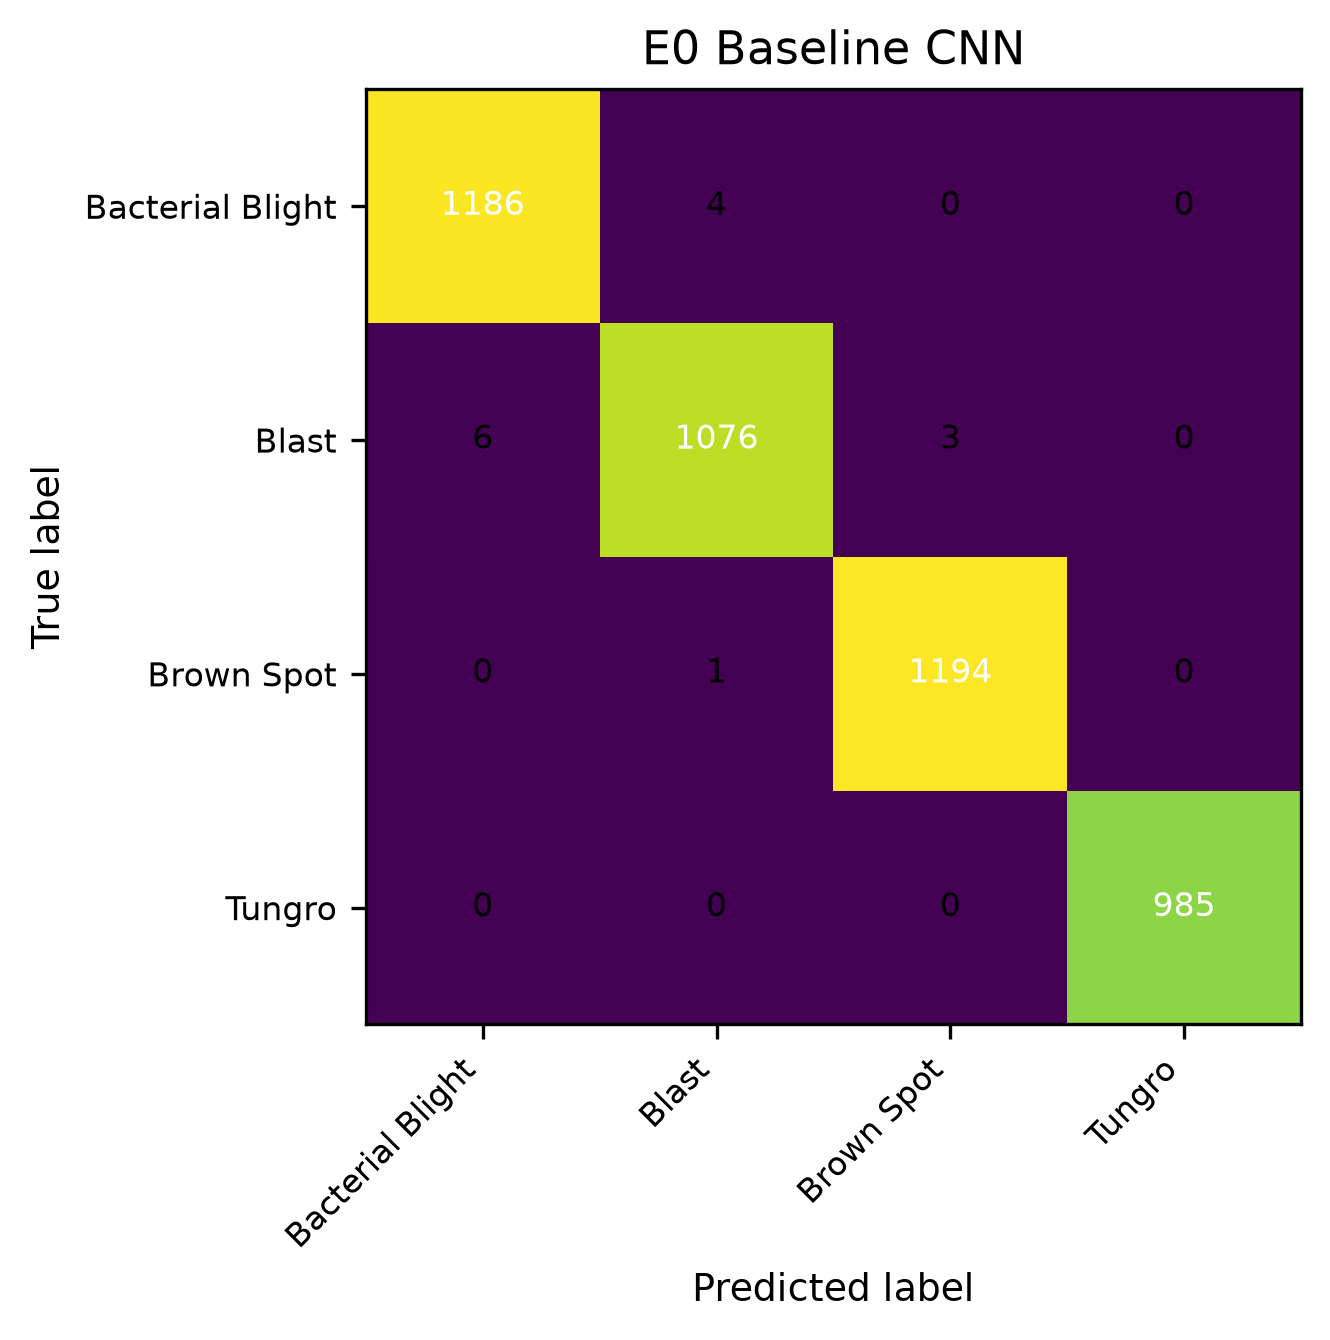
\includegraphics[width=\linewidth]{figures/fig03_aggregate_confusion_e0.png}
\centerline{(a) E0 baseline CNN}
\end{minipage}
\hfill
\begin{minipage}{0.32\textwidth}
\centering
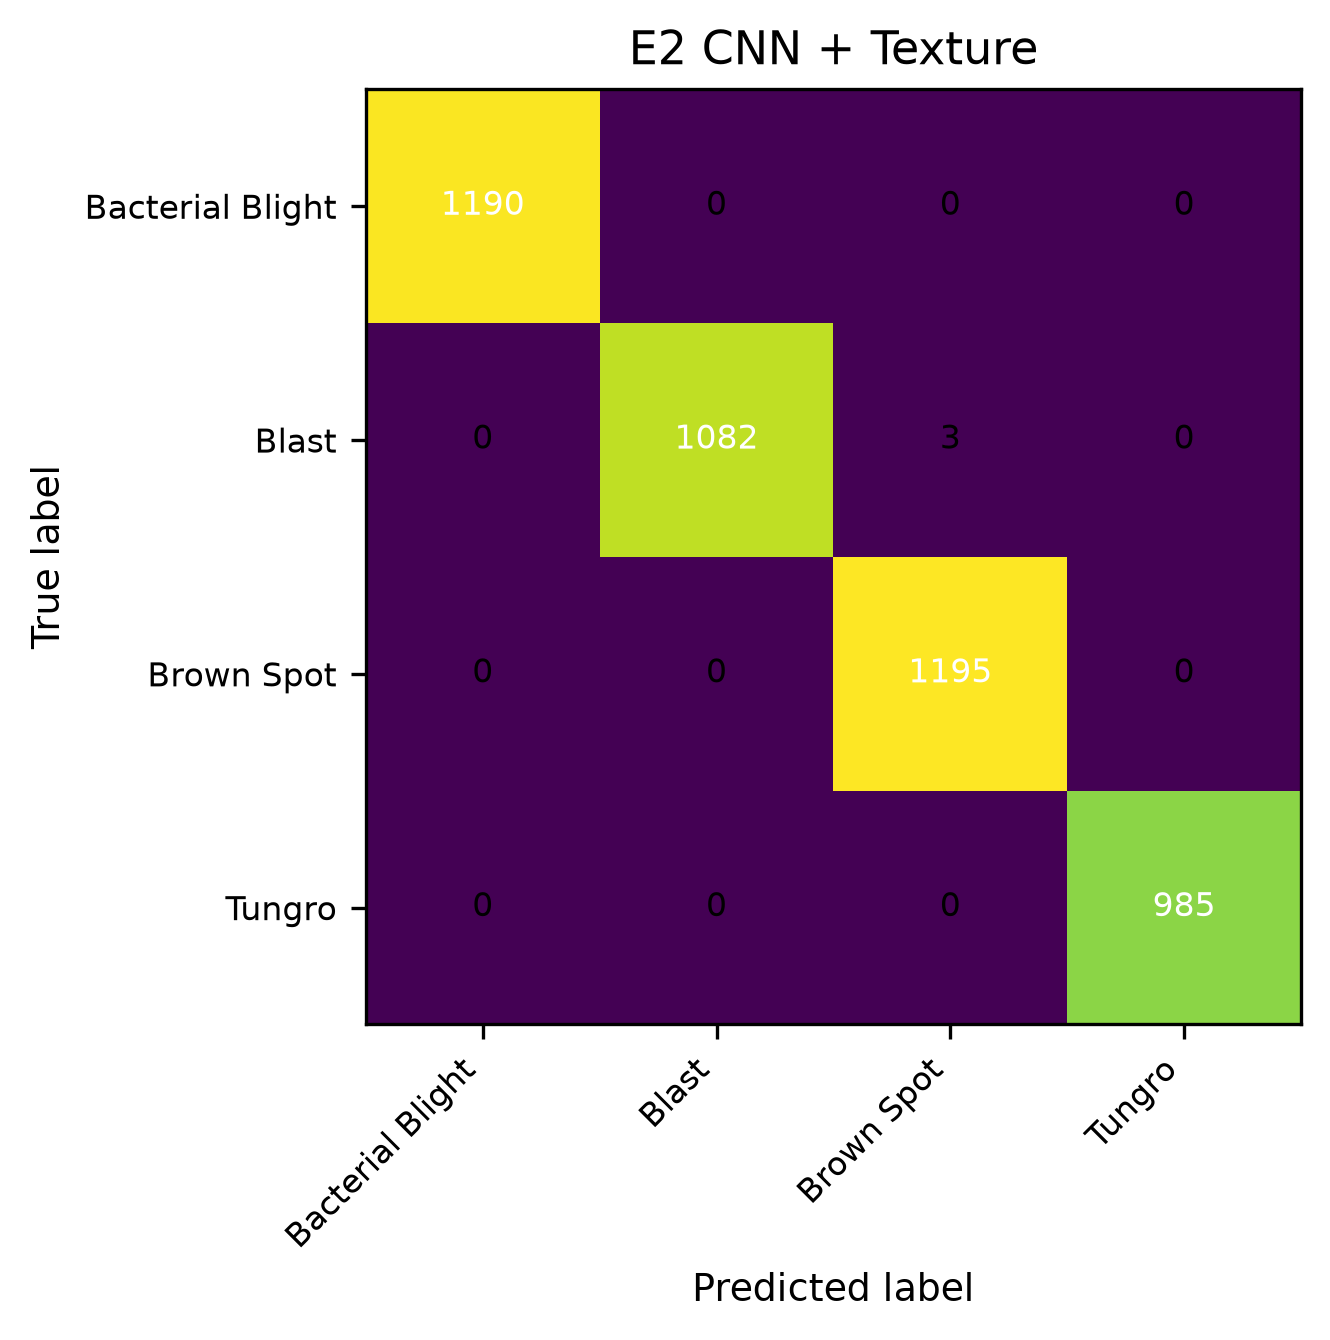
\includegraphics[width=\linewidth]{figures/fig04_aggregate_confusion_e2.png}
\centerline{(b) E2 CNN + texture}
\end{minipage}
\hfill
\begin{minipage}{0.32\textwidth}
\centering
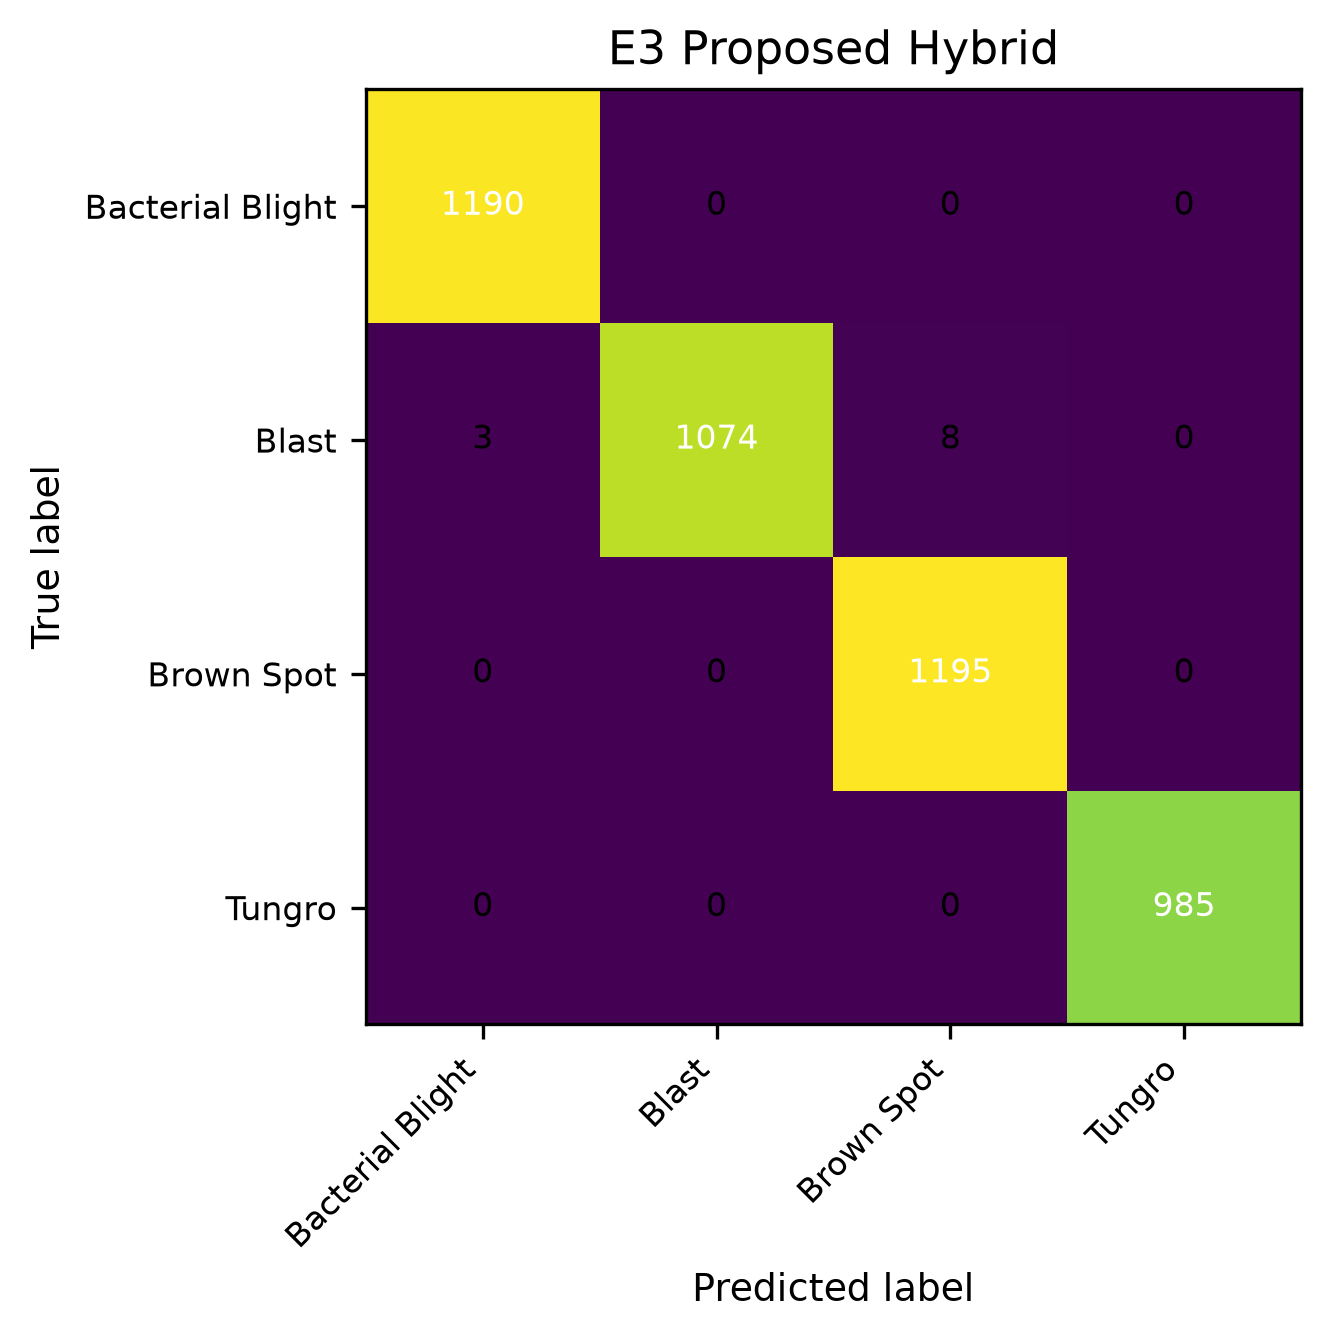
\includegraphics[width=\linewidth]{figures/fig05_aggregate_confusion_e3.png}
\centerline{(c) E3 proposed hybrid}
\end{minipage}
\caption{Aggregate confusion matrices over five seeds. Each matrix summarizes 4,455 predictions. E0 is shown as the baseline, E2 as the best average model, and E3 as the proposed segmentation-texture hybrid model.}
\label{fig:aggregate_confusion_matrices}
\end{figure*}

\section{Discussion}

The results show that the evaluated dataset remains highly separable even after controlling visually equivalent samples through perceptual-hash grouping. The baseline MobileNetV2 model already achieved a high macro-F1 score of $0.9969 \pm 0.0052$, which indicates a performance saturation scenario. Under this condition, the margin for measurable improvement is small, and additional components do not necessarily produce statistically significant gains.

The strongest configuration was E2, which fused MobileNetV2 embeddings with explicit GLCM+DWT descriptors extracted from the original images. This model obtained the highest mean macro-F1 ($0.9993 \pm 0.0015$) and the lowest number of aggregate errors across five seeds. This result is consistent with previous works showing that handcrafted texture, color, and frequency descriptors can capture useful visual information for rice disease classification \cite{sutikno2026glcm_lbp_color,prity2026ffnn}. In this study, however, these descriptors were not evaluated as a standalone classifier input, but as a complementary branch fused with a lightweight CNN.

The segmentation-only configuration, E1, achieved the lowest inference time while maintaining high classification performance. This suggests that removing background regions can simplify the visual input and improve efficiency without substantially reducing discriminative information. This finding is aligned with segmentation-aware rice disease classification approaches, where region-focused processing helps the classifier attend to relevant leaf areas \cite{shakeel2026contour}. Nevertheless, in the present ablation, segmentation alone produced only a small average improvement over the baseline and did not reach statistical significance.

The proposed hybrid model, E3, was competitive but did not outperform E2 or show a statistically significant improvement over E0. This can be explained by three main factors. First, the baseline was already very strong, leaving little room for additional gains. Second, segmentation may remove not only irrelevant background but also some contextual or boundary information useful for classification. Third, the segmented CNN input and the texture descriptors may provide partially redundant information, limiting the benefit of their fusion. Therefore, E3 improves over the baseline in aggregate accuracy, but its added complexity does not translate into a clear performance advantage.

Compared with recent CNN-based rice disease classification studies, the results confirm that transfer learning backbones can achieve strong performance in this task \cite{ismail2026densenet}. However, direct numerical comparison with prior works should be interpreted cautiously because datasets, splits, preprocessing strategies, leakage controls, and evaluation protocols differ across studies. The main contribution of this paper is therefore not a claim of absolute superiority over previous models, but a controlled comparison of segmentation, explicit texture fusion, and their combination under the same experimental conditions.

Several threats to validity remain. First, the pHash-based split reduced the risk of exact or near-exact visual leakage by keeping images with the same perceptual hash within the same split. However, this procedure does not guarantee the removal of all visually or semantically similar samples, such as images captured under the same background, lighting, leaf position, or acquisition session. Second, the evaluation used one fixed pHash-controlled train/validation/test split and five random seeds. Therefore, the multi-seed evaluation measures training stability under the same data partition, while sensitivity to alternative dataset partitions was not evaluated. Third, no external field-acquired dataset was included; therefore, the reported performance should be interpreted within the conditions of the evaluated public dataset and not as direct evidence of generalization to uncontrolled agricultural environments. Finally, the segmentation method was based on classical L*a*b* Otsu thresholding, which is simple and reproducible, but may be less robust when images contain complex backgrounds, shadows, overlapping leaves, or lighting variations.

Overall, the evidence suggests that explicit texture fusion was the most effective enhancement in this experimental setting, segmentation was the most efficient configuration, and the proposed segmentation-texture hybrid was competitive but not statistically superior. Future work should validate the same ablation design on external field-acquired datasets to determine whether segmentation and texture fusion provide larger benefits under stronger domain shift.

\section{Conclusions}

This study evaluated the contribution of segmentation and explicit texture descriptors in lightweight CNN-based rice leaf disease classification through a controlled ablation design. The results show that the proposed segmentation-texture hybrid approach is feasible and competitive, but it was not the strongest configuration in the evaluated setting. Across five random seeds, the CNN with explicit GLCM+DWT texture fusion (E2) achieved the highest mean macro-F1 score, while the segmentation-only model (E1) achieved the lowest inference time. The proposed hybrid model (E3) improved over the baseline in aggregate accuracy, but it did not produce a statistically significant advantage over the baseline or outperform the texture-fusion configuration.

The main empirical finding is that, under a pHash-controlled split, explicit texture features provided the most consistent performance gain, whereas segmentation mainly contributed to efficiency. This suggests that handcrafted texture and frequency descriptors can still complement CNN embeddings in rice leaf disease classification, especially when symptoms are visually expressed through lesions, spots, and local texture patterns. However, the high baseline performance indicates that the dataset presents a performance saturation scenario, where additional components may not produce proportional or statistically significant improvements.

Therefore, the contribution of this work lies not in claiming absolute superiority of the proposed hybrid model, but in providing a controlled comparison of four configurations under the same split, training setup, metrics, and seeds. This ablation evidence helps clarify the relative effect of segmentation, texture fusion, and their combination in a lightweight CNN pipeline.

Future work should validate the same experimental design on external and field-acquired datasets with more diverse lighting conditions, backgrounds, cameras, and disease stages. Additional work should also explore stronger near-duplicate grouping strategies, explainability methods such as Grad-CAM, and real-time deployment evaluation on resource-constrained devices. These extensions would help determine whether segmentation and texture fusion provide larger benefits under stronger domain shift and practical agricultural conditions.

\section{Reproducibility and Artifacts}

The source code, configuration files, experimental scripts, and generated artifacts are available in the public repository: \url{https://github.com/Piero010405/rice-leaf-hybrid-cnn_psa}. The Rice Leaf Disease Images dataset used in this study is publicly available on Kaggle \cite{kaggle_rice_leaf_disease}; the original images are not redistributed in the repository and must be downloaded from the original source.

The repository includes the implementation of the four experimental scenarios, the pHash-controlled split generation, configuration files, multi-seed training scripts, generated tables, figures, classification reports, prediction files, aggregate confusion matrices, and the LaTeX source of the paper. All experiments used the same pHash-controlled train/validation/test split, batch size of 8, and five random seeds: 7, 42, 99, 123, and 2026.

\section*{Acknowledgment}

The author thanks Universidad San Ignacio de Loyola and Dr. Manuel Augusto Yarleque Medina, instructor of the course Mathematics Applied to Computing, for providing the academic context in which this experimental study was developed.

\balance
\bibliographystyle{IEEEtran}
\bibliography{bib/references}

\end{document}
